\documentclass[
11pt, % The default document font size, options: 10pt, 11pt, 12pt
codirector, % Uncomment to add a codirector to the title page
]{charter} 

\usepackage{enumitem}


% El títulos de la memoria, se usa en la carátula y se puede usar el cualquier lugar del documento con el comando \ttitle
\titulo{Tester para amplificador de fibra óptica} 

% Nombre del posgrado, se usa en la carátula y se puede usar el cualquier lugar del documento con el comando \degreename
\posgrado{Carrera de Especialización en Sistemas Embebidos} 
%\posgrado{Carrera de Especialización en Internet de las Cosas} 
%\posgrado{Carrera de Especialización en Intelegencia Artificial}
%\posgrado{Maestría en Sistemas Embebidos} 
%\posgrado{Maestría en Internet de las cosas}

% Tu nombre, se puede usar el cualquier lugar del documento con el comando \authorname
\autor{Lucas Constantino} 

% El nombre del director y co-director, se puede usar el cualquier lugar del documento con el comando \supname y \cosupname y \pertesupname y \pertecosupname
\director{Nombre del Director}
\pertenenciaDirector{pertenencia} 
% FIXME:NO IMPLEMENTADO EL CODIRECTOR ni su pertenencia
\codirector{John Doe} % para que aparezca en la portada se debe descomentar la opción codirector en el documentclass
\pertenenciaCoDirector{FIUBA}

% Nombre del cliente, quien va a aprobar los resultados del proyecto, se puede usar con el comando \clientename y \empclientename
\cliente{Nicolas Casco}
\empresaCliente{Skyloom Global}

% Nombre y pertenencia de los jurados, se pueden usar el cualquier lugar del documento con el comando \jurunoname, \jurdosname y \jurtresname y \perteunoname, \pertedosname y \pertetresname.
\juradoUno{Nombre y Apellido (1)}
\pertenenciaJurUno{pertenencia (1)} 
\juradoDos{Nombre y Apellido (2)}
\pertenenciaJurDos{pertenencia (2)}
\juradoTres{Nombre y Apellido (3)}
\pertenenciaJurTres{pertenencia (3)}
 
\fechaINICIO{1 de Marzo de 2022}		%Fecha de inicio de la cursada de GdP \fechaInicioName
\fechaFINALPlan{18 de junio de 2022} 		%Fecha de final de cursada de GdP
\fechaFINALTrabajo{13 de Marzo de 2023}	%Fecha de defensa pública del trabajo final


\begin{document}

\maketitle
\thispagestyle{empty}
\pagebreak


\thispagestyle{empty}
{\setlength{\parskip}{0pt}
\tableofcontents{}
}
\pagebreak


\section*{Registros de cambios}
\label{sec:registro}


\begin{table}[ht]
\label{tab:registro}
\centering
\begin{tabularx}{\linewidth}{@{}|c|X|c|@{}}
\hline
\rowcolor[HTML]{C0C0C0} 
Revisión & \multicolumn{1}{c|}{\cellcolor[HTML]{C0C0C0}Detalles de los cambios realizados} & Fecha      \\ \hline
1.0	& Creación del documento.				& 01/03/2022 \\ \hline
1.1	& Se completan las secciones 1 a 5 inclusive		& 15/03/2022 \\ \hline
1.2	& Se completan las secciones 6 a 9 inclusive                & 22/03/2022 \\ \hline
1.3     & Se completan las secciones 10 a 12 inclusive		& 29/03/2022 \\ \hline
1.4	& Se completan las secciones 13 a 15 inclusive		& 05/04/2022 \\ \hline
%		  En distintas líneas \newline
%		  Así                                                    & dd/mm/aaaa \\ \hline
%3      & Se completa hasta el punto 11 inclusive                & dd/mm/aaaa \\ \hline
%4      & Se completa el plan	                                 & dd/mm/aaaa \\ \hline
\end{tabularx}
\end{table}

\pagebreak



\section*{Acta de constitución del proyecto}
\label{sec:acta}

\begin{flushright}
Buenos Aires, \fechaInicioName
\end{flushright}

\vspace{2cm}

Por medio de la presente se acuerda con el Ing. \authorname\hspace{1px} que su Trabajo Final de la \degreename\hspace{1px} se titulará ``\ttitle'', consistirá esencialmente en el desarrollo y construcción de un dispositivo integrado capaz de monitorear y controlar un amplificador de fibra óptica, y tendrá un presupuesto preliminar estimado de 642 hs de trabajo y US\$ 732, con fecha de inicio \fechaInicioName\hspace{1px} y fecha de presentación pública \fechaFinalName.

Se adjunta a esta acta la planificación inicial.

\vfill

% Esta parte se construye sola con la información que hayan cargado en el preámbulo del documento y no debe modificarla
\begin{table}[ht]
\centering
\begin{tabular}{ccc}
\begin{tabular}[c]{@{}c@{}}Ariel Lutenberg \\ Director posgrado FIUBA\end{tabular} & \hspace{2cm} & \begin{tabular}[c]{@{}c@{}}\clientename \\ \empclientename \end{tabular} \vspace{2.5cm} \\ 
\multicolumn{3}{c}{\begin{tabular}[c]{@{}c@{}} \supname \\ Director del Trabajo Final\end{tabular}} \vspace{2.5cm} \\
%\begin{tabular}[c]{@{}c@{}}\jurunoname \\ Jurado del Trabajo Final\end{tabular}     &  & \begin{tabular}[c]{@{}c@{}}\jurdosname\\ Jurado del Trabajo Final\end{tabular}  \vspace{2.5cm}  \\
%\multicolumn{3}{c}{\begin{tabular}[c]{@{}c@{}} \jurtresname\\ Jurado del Trabajo Final\end{tabular}} \vspace{.5cm}                                                                     
\end{tabular}
\end{table}




\section{1. Descripción técnica-conceptual del proyecto a realizar}
\label{sec:descripcion}

Un EDFA (Erbuim-Doped Fiber Amplifier) es un dispositivo optoelectrónico que permite amplificar una señal lumínica transportada mediante una fibra óptica desde una potencia del orden de 1 mW hasta aproximadamente 1 W (unas mil veces). Estos amplificadores se usan particularmente en las bandas L y C del espectro de longitud de onda para compensar las pérdidas en la fibra óptica en comunicaciones de gran distancia.

En general, un EDFA además de contar con una entrada y una salida de fibra óptica tiene un microcontrolador interno encargado de controlar el proceso de amplificación. Para poder comunicarse con el exterior este cuenta con un puerto para la conexión de varias señales, entre ellas la tensión de alimentación (potencia) para la amplificación propiamente dicha y otras señales de entrada y salida tanto analógicas como digitales, que describen el estado del amplificador, valores de ciertos parámetros y una interfaz serie que permite establecer una comunicación con el dispositivo maestro que lo comandará.

El dispositivo a desarrollar debe poder conectarse directamente al puerto de un EDFA del fabricante Nuphoton, proveer la corriente necesaria para que funcione, medirla y presentarle al usuario de forma clara este valor y el resto de los parámetros relevantes recibidos. Para esto debe contar con un display LCD táctil que además permita enviarle comandos al amplificador.

Por otro lado, como el amplificador es un dispositivo muy caro que ademas formará parte de una terminal de comunicación óptica satelital destinada a volar, es imperativo que se tomen las medidas necesarias para evitar dañarlo durante la etapa de integración, tanto mecánica como electricamente. Por dicha razón el dispositivo debe contar con las protecciones eléctricas pertinentes.

En la Figura \ref{fig:diagTester} se presenta el diagrama en bloques del sistema. Se observa que este consta de un microcontrolador como controlador central al cual se encuentran conectados todo el resto de los periféricos e interfaces. Ademas aclara que el EDFA, la PC y la fuente de alimentación externa no forman parte del dispositivo a desarrollar, solamente se encuentran conectados a este mediante algun tipo de interfaz.


\begin{figure}[H]
\centering 
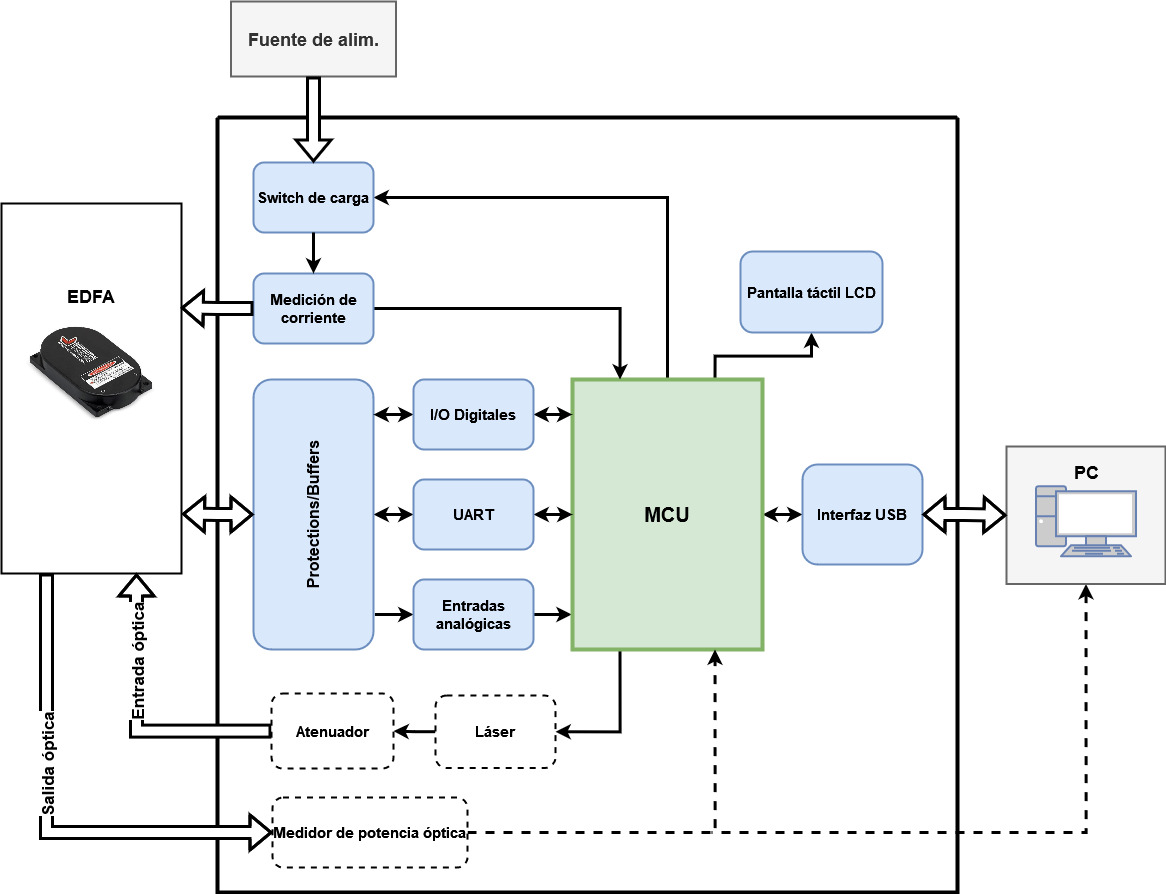
\includegraphics[width=0.75\textwidth]{./Figuras/diagTester.jpg}
\caption{Diagrama en bloques del sistema}
\label{fig:diagTester}
\end{figure}


Si bien el fabricante del EDFA ofrece una placa para establecer una comunicación entre el EDFA y una PC, ademas de ser costosa y no funcionar del todo correctamente, esta no cuenta con la conexión de todas las señales por lo que hace que conocer el estado exacto de todas las señales y parámetros lleve mucho tiempo y requiera una computadora. El presente proyecto se destaca especialmente por incorporar todos los componentes necesarios para poder monitorear y comandar de forma segura este tipo de amplificadores en un solo dispositivo, presentando al usuario los parámetros relevantes del EDFA y su consumo de corriente sin la necesidad de una PC.

Este equipo se enmarca como uno de los denominados Equipamiento Eléctrico de Soporte en Tierra perteneciente al departamento de Ensamble, Integración y Testing de la empresa Skyloom Global y será utilizado tanto durante la etapa de desarrollo como de ensamble de lotes de terminales ópticas satelitales para órbita LEO.


\section{2. Identificación y análisis de los interesados}
\label{sec:interesados}


\begin{table}[ht]
%\caption{Identificación de los interesados}
%\label{tab:interesados}
\begin{tabularx}{\linewidth}{@{}|l|X|X|l|@{}}
\hline
\rowcolor[HTML]{C0C0C0} 
Rol           & Nombre y Apellido & Organización 	& Puesto 	\\ \hline
Cliente       & \clientename      &\empclientename	& Jefe de Proyecto	\\ \hline
Responsable   & \authorname       & FIUBA        	& Alumno 	\\ \hline
Orientador    & \supname	      & \pertesupname 	& Director Trabajo final \\ \hline
%Equipo        & - &              	&        	\\ \hline
Usuario final & -                 & Skyloom Global	& Dpto. de Integración y Testing	\\ \hline
\end{tabularx}
\end{table}

Características de los interesados:
\begin{itemize}
	\item Cliente: es exigente con la presentación del producto y el cumplimiento de sus requerimientos. También puede ayudar a definir los requerimientos.
\end{itemize}


\section{3. Propósito del proyecto}
\label{sec:proposito}

El propósito de este proyecto es desarrollar un dispositivo integrado capaz de proveer al usuario una forma sencilla de monitorear y comandar un EDFA, sin necesidad de usar una computadora. De esta forma el dispositivo se utilizará en dos instancias bien definidas: la primera es durante el desarrollo de nuevos modelos de terminales opticas satelitales y la segunda es durante la integración de grandes lotes para su fabricación en masa.

\section{4. Alcance del proyecto}
\label{sec:alcance}

Este proyecto queda delimitado por:
\begin{itemize}
	\item Diseño y construcción de un dispositivo funcional de un tester que consta de hardware y software.
	\item Diseño y ensamble del PCB del dispositivo.
	\item Integración completa del dispositivo en soporte mecánico.
	\item Verificación funcional del producto final.
	\item Simulación de funcionamiento de hardware mediante software apropiado.
	\item Diseño e implementación de la arquitectura de software del dispositivo.
	\item Diseño e implementación del software a ejecutarse en la PC.
	\item Documentación de diseño para su producción y manual de uso.
\end{itemize}

Por otro lado, queda excluído del presente proyecto:
\begin{itemize}
	\item Fabricación del PCB del dispositivo.
	\item Especificación de las pruebas a ejecutar sobre el amplificador óptico utilizando el dispositivo.
	\item Procesamiento e interpretación de los valores de los parámetros enviados por el EDFA.
	\item Diseño y construcción de la fuente de alimentación externa.
\end{itemize}


\section{5. Supuestos del proyecto}
\label{sec:supuestos}

Para el desarrollo del presente proyecto se supone que:
\begin{itemize}
	\item El cliente proveerá una versión inicial de la placa del dispositivo final para desarrollo.
	\item Se podrá contar con los insumos necesarios en tiempo y forma.
	\item El cliente posee las instalaciones e instrumental necesario para realizar mediciones y ensayos.
	\item Se dispondrá del tiempo necesario para el desarrollo del proyecto.
	\item Se cuenta con toda la información técnica acerca del amplificador óptico, sus parámetros y funcionamiento.
	\item Se contará con un EDFA o con una placa electrónica que simule su comportamiento.
	\item El contexto macroeconómico permitirá mantener al proyecto económicamente viable durante toda su duración.
	\item El dispositivo le seguirá siendo necesario al cliente al momento de la finalización del proyecto.
\end{itemize}

\section{6. Requerimientos}
\label{sec:requerimientos}

Los requerimientos del proyecto se definieron luego de acordarlos con el cliente y considerando las sugerencias de los posibles usuarios finales. Estos se detallan a continuación, agrupados en distintas secciones y en orden de prioridad decreciente.

\begin{enumerate}
	\item Requerimientos generales
		\begin{enumerate}
			\item Todos los entregables del proyecto deben estar terminados y listos para presentarse el día 13 de Marzo de 2023.
			\item Todos los componentes del dispositivo, a excepción de la fuente de alimentación, deben estar montados sobre una misma carcasa de material no conductor.
			\item El dispositivo debe poder conectarse a la red de 110V/60Hz mediante una fuente de alimentación externa.
			\item El dispositivo, sin la fuente de alimentaciön externa, no debe pesar mas de 750 g y no debe tener mas de 15 cm de largo, 10 cm de ancho y 6 cm de alto.
			\item El dispositivo debe conectarse al EDFA mediante un cable con conectores Micro-D.
		\end{enumerate}
	\item Requerimientos funcionales
		\begin{enumerate}
			\item Requerimientos de hardware
				\begin{enumerate}[label*=\arabic*.]
					\item Todas las señales eléctricas entrantes y salientes del EDFA deben estar aisladas y protegidas contra descargas electrostáticas.
					\item El dispositivo debe contar con una pantalla táctil y mostrar en ella el estado de todas las señales del EDFA y los valores de sus parámetros.
					\item El dispositivo debe poder medir el consumo de corriente del EDFA con una precisión del 10\%.
					\item El dispositivo debe desconectar la alimentación del EDFA de forma automática si el consumo de corriente supera el valor establecido por el usuario. Este valor debe ser configurable por el usuario mediante la pantalla táctil.
					\item El dispositivo debe poder medir el nivel de tensión de alimentación del EDFA con una precisión del 10\%.
					\item El dispositivo debe desconectar la alimentación del EDFA de forma automática si el nivel de tensión cae por debajo del valor establecido por el usuario. Este valor debe ser configurable por el usuario mediante la pantalla táctil.
					\item El dispositivo debe poder conectarse a una computadora mediante USB.
				\end{enumerate}
			\item Requerimientos de firmware
				\begin{enumerate}[label*=\arabic*.]
					\item El dispositivo debe utilizar un sistema operativo en tiempo real.
					\item El dispositivo debe establecer una comunicación con el EDFA para el envío de comandos mediante una interfaz UART.
					\item Cuando el dispositivo se encuentra conectado a una computadora el usuario debe poder, mediante una consola, configurar los mismos parámetros que en la pantalla táctil y además, establecer una comunicación directa con el EDFA.
					\item El dispositivo debe actualizar la información mostrada en la pantalla al menos cada 0.5 segundos.
					\item El dispositivo debe interpretar las señales analógicas de entrada, procesarlas y mostrarlas en la pantalla.
				\end{enumerate}
		\end{enumerate}
	\item Requerimientos no funcionales
		\begin{enumerate}
			\item Se deberá generar la documenatación correspondiente.
			\item El dispositivo no debe generar ni emanar ningún tipo de partículas o residuo.
			\item El dispositivo debe cumplir con la normativa vigente de compatibilidad electromagnética.
			\item El dispositivo no debe generar temperaturas superiores a 40°C.
		\end{enumerate}
	\item Requerimientos de testing
		\begin{enumerate}
			\item Test de consumo de corriente del EDFA.
			\item Test de desconexión de alimentación del EDFA por sobrecorriente.
			\item Test de comunicación UART con EDFA.
			\item Test de nivel de tensión de alimentación del EDFA.
			\item Test de desconexión de alimentación del EDFA por caída de tensión.
			\item Test de uso del dispositivo mediante una computadora.
		\end{enumerate}
	\item Requerimientos opcionales
		\begin{enumerate}
			\item El dispositivo podría contar con un software de PC con interfaz gráfica para el manejo de la comunicación con el EDFA y el monitoreo de señales.
		\end{enumerate}
\end{enumerate}

% Faltaria poner los requerimientos de regulaciones y normas vigentes

\section{7. Historias de usuarios (\textit{Product backlog})}
\label{sec:backlog}

Se dará una visión de las funcionalidades esperadas por los distintos usuarios del producto. A cada
historia se le asocia un grado de ponderación de acuerdo al nivel de importancia de la característica mencionada y una prioridad
respecto al resto.


Para la ponderación se usarán tres niveles: 1, 3 y 7. 
Para la prioridad se usará de 1 a 5, siendo 1 la prioridad mas baja.

\begin{enumerate}
	\item Como ingeniero de desarrollo desearía poder saber el consumo de corriente del EDFA cuando está funcionando activamente sobre una señal óptica para poder calcular su eficiencia.
	\begin{itemize}
		\item Ponderación: 7
		\item Prioridad: 3
	\end{itemize}
	\item Como técnico de integración desearía poder probar todas las señales del EDFA rápidamente para realizar una aceptación de lote en poco tiempo.
	\begin{itemize}
		\item Ponderación: 7
		\item Prioridad: 5
	\end{itemize}
	\item Como ingeniero de desarrollo desearía poder contar con un dispositivo integrado que indique todos los parámetros internos del EDFA para poder monitorear su performance, sin necesidad de usar una computeadora u otro instrumento.
	\begin{itemize}
		\item Ponderación: 3
		\item Prioridad: 4
	\end{itemize}
	\item Como técnico de integración desearía poder enviarle comandos al EDFA para simular que se encuentra conectado a un dispositivo que lo controla, y asi observar su comportamiento.
	\begin{itemize}
		\item Ponderación: 1
		\item Prioridad: 2
	\end{itemize}
	\item Como ingeniero de desarrollo desearía que el dispositivo cuente con las medidas de protección necesarias tanto como para evitar dañar equipos de vuelo como para poder utilizarlo dentro de una sala limpia.
	\begin{itemize}
		\item Ponderación: 3
		\item Prioridad: 2
	\end{itemize}
\end{enumerate}

\section{8. Entregables principales del proyecto}
\label{sec:entregables}

Se incluyen los siguientes entregables:

\begin{itemize}
	\item Manual de uso del dispositivo
	\item Diagramas de circuitos esquemáticos
	\item Código fuente del firmware
	\item Reporte de ensayos
	\item Producto final funcional
	\item Memoria del proyecto
\end{itemize}

\section{9. Desglose del trabajo en tareas}
\label{sec:wbs}

Se presenta a continuación el WBS del proyecto mediante una lista indexada, detallando las actividades a realizar en cada sección y su duración correspondiente.

\begin{enumerate}
\item Planificación del proyecto (50 hs)
	\begin{enumerate}
	\item Definición de alcance y requerimientos con el cliente (12 hs)
	\item Análisis de factibilidad técnico-económica (8 hs)
	\item Confección del plan de trabajo (30 hs)
	\end{enumerate}
\item Análisis preliminar (32 hs)
	\begin{enumerate}
	\item Estudio detallado del funcionamiento del EDFA (12 hs)
	\item Elección del microcontrolador (8 hs)
	\item Selección de los principales componentes a utilizar (12 hs)
	\end{enumerate}
\item Diseño general del dispositivo (50 hs)
	\begin{enumerate}
	\item Construcción de diagrama en bloques (12 hs)
	\item Definición de interfaces (6 hs)
	\item Diseño y fabricación de placa de desarrollo (32 hs)
	\end{enumerate}
\item Diseño de hardware (122 hs)
	\begin{enumerate}
	\item Diseño del diagrama esquemático (30 hs)
	\item Diseño del PCB (24 hs)
	\item Ensamble del PCB (12 hs)
	\item Puesta en marcha del PCB (12 hs)
	\item Ejecución de retrabajos del PCB (6 hs)
	\item Diseño de la carcasa (20 hs)
	\item Impresión de la carcasa (12 hs)
	\item Integración y montaje del dispositivo completo (6 hs)
	\end{enumerate}
\item Diseño de firmware (140 hs)
	\begin{enumerate}
	\item Definición de la arquitectura (14 hs)
	\item Modularización del código (20 hs)
	\item Desarrollo de la interfaz de usuario en pantalla táctil (30 hs)
	\item Desarrollo del monitoreo y protección de corriente (10 hs)
	\item Desarrollo del monitoreo y protección de tensión (10 hs)
	\item Desarrollo de la interfaz UART (26 hs)
	\item Desarrollo de la interfaz USB (30 hs)
	\end{enumerate}
\item Verificación y validación (146 hs)
	\begin{enumerate}
	\item Pruebas de campo (32 hs)
	\item Pruebas de la interfaz de usuario (14 hs)
	\item Pruebas del monitor de corriente (10 hs)
	\item Pruebas de la protección de corriente (10 hs)
	\item Pruebas del monitor de tensión (10 hs)
	\item Pruebas de la protección de tensión (10 hs)
	\item Pruebas de la interfaz UART (20 hs)
	\item Pruebas de la interfaz USB (20 hs)
	\item Corrección de errores del firmware (20 hs)
	\end{enumerate}
\item Documentación (102 hs)
	\begin{enumerate}
	\item Elaboración del manual de usuario (32 hs)
	\item Elaboración de la memoria técnica (40 hs)
	\item Elaboración de la presentación pública del proyecto (30 hs)
	\end{enumerate}
\end{enumerate}

Cantidad total de horas: (642 hs)

\section{10. Diagrama de Activity On Node}
\label{sec:AoN}

A continuación se presenta el diagrama de actividades Activity On Node. La duración de las tareas se encuentran expresadas en horas y el camino crítico del proyecto indicado mediante las flechas de mayor espesor.

Para mayor claridad del diagrama, las tareas 5, 6 y 7 se encuentran reducidas en una sola instancia ya que sus actividades de menor nivel se ejecutan de forma secuencial.

\begin{figure}[H]
\centering 
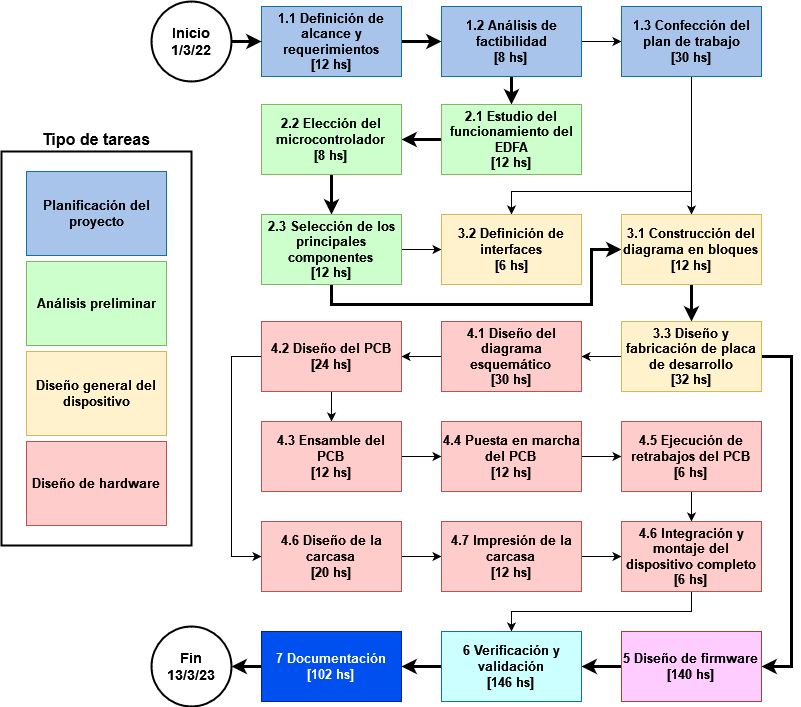
\includegraphics[width=.9\textwidth]{./Figuras/AoN.png}
\caption{Diagrama de \textit{Activity on Node}}
\label{fig:AoN}
\end{figure}

\section{11. Diagrama de Gantt}
\label{sec:gantt}

En la figura 3 se muestran las tareas con sus respectivas fechas iniciales y finales. Para la duración de los días se estimó una jornada de trabajo de 9 horas por semana (de 5 días hábiles).

\begin{figure}[H]
\centering 
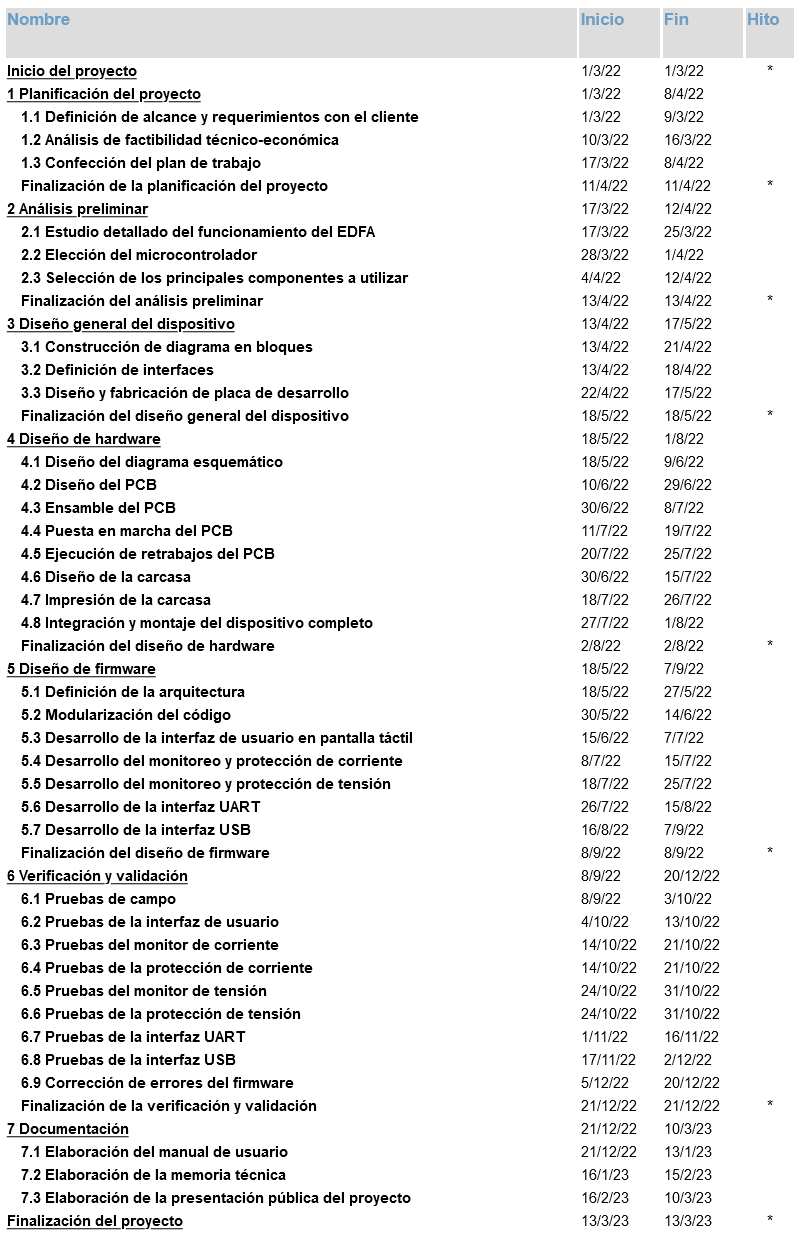
\includegraphics[width=.85\textwidth]{./Figuras/Gantt_Tareas.png}
\caption{Diagrama de \textit{Tareas del diagrama de Gantt}}
\label{fig:Gantt_Tareas}
\end{figure}

\begin{figure}[htpb]
\centering 
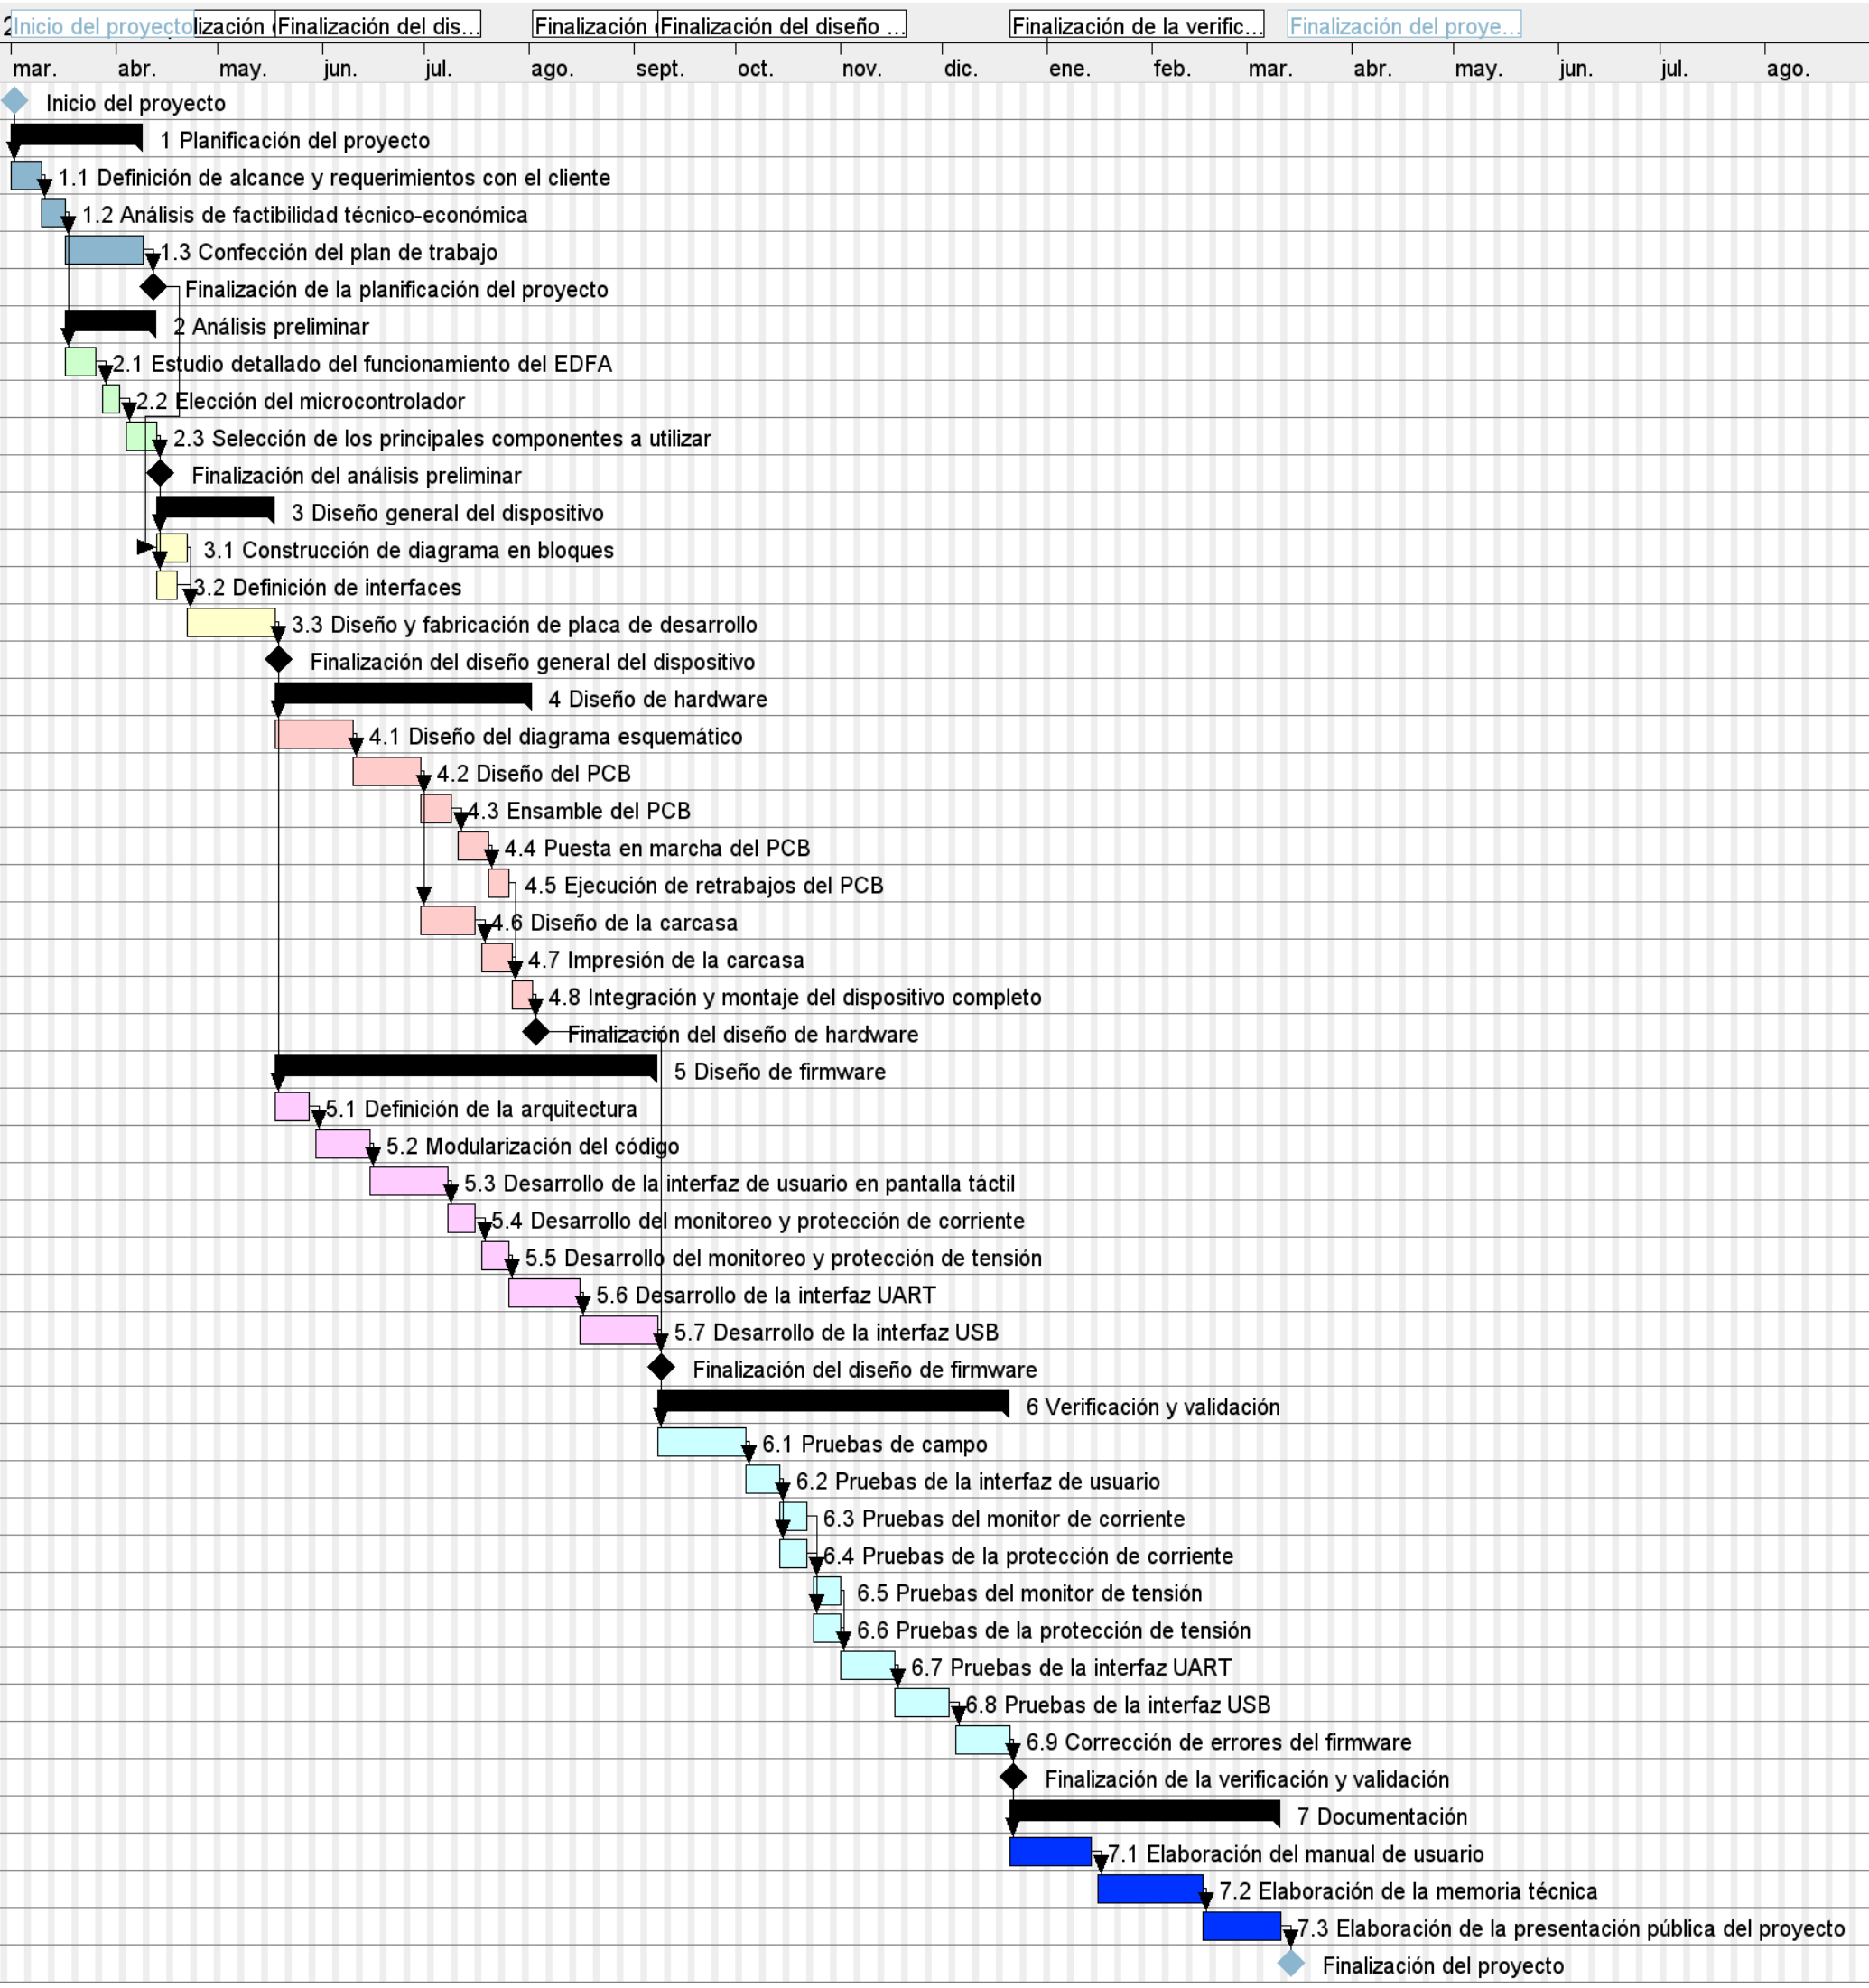
\includegraphics[height=.7\textheight]{./Figuras/Gantt_Diag.png}
\caption{Diagrama de Gantt}
\label{fig:Gantt_Diag}
\end{figure}

\section{12. Presupuesto detallado del proyecto}
\label{sec:presupuesto}

A continuación se muestra una tabla detallando los costos que surgen del desarrollo del proyecto. Los valores se encuentran expresados en dólares estadounidenses.

\begin{table}[H]
\centering
\begin{tabularx}{\linewidth}{@{}|X|c|r|r|@{}}
\hline
\rowcolor[HTML]{C0C0C0} 
\multicolumn{4}{|c|}{\cellcolor[HTML]{C0C0C0}COSTOS DIRECTOS} \\ \hline
\rowcolor[HTML]{C0C0C0} 
Descripción &
  \multicolumn{1}{c|}{\cellcolor[HTML]{C0C0C0}Cantidad} &
  \multicolumn{1}{c|}{\cellcolor[HTML]{C0C0C0}Valor unitario} &
  \multicolumn{1}{c|}{\cellcolor[HTML]{C0C0C0}Valor total} \\ \hline
Fabricación de PCB de placa de desarrollo &
  \multicolumn{1}{c|}{5} &
  \multicolumn{1}{c|}{\$25*} &
  \multicolumn{1}{c|}{\$125} \\ \hline
Placa de desarrollo STM32F429 &
  \multicolumn{1}{c|}{1} &
  \multicolumn{1}{c|}{\$25} &
  \multicolumn{1}{c|}{\$25} \\ \hline
Display LCD &
  \multicolumn{1}{c|}{1} &
  \multicolumn{1}{c|}{\$9} &
  \multicolumn{1}{c|}{\$9} \\ \hline
Fuente de alimentación externa &
  \multicolumn{1}{c|}{1} &
  \multicolumn{1}{c|}{\$30*} &
  \multicolumn{1}{c|}{\$30} \\ \hline
Componentes electrónicos varios** &
  \multicolumn{1}{c|}{1} &
  \multicolumn{1}{c|}{\$170*} &
  \multicolumn{1}{c|}{\$170} \\ \hline
Filamento PLA &
  \multicolumn{1}{c|}{1} &
  \multicolumn{1}{c|}{\$22} &
  \multicolumn{1}{c|}{\$22} \\ \hline
Fabricación de PCB de dispositivo terminado &
  \multicolumn{1}{c|}{5} &
  \multicolumn{1}{c|}{\$25*} &
  \multicolumn{1}{c|}{\$125} \\ \hline
Componentes cable dispositivo a EDFA &
  \multicolumn{1}{c|}{1} &
  \multicolumn{1}{c|}{\$86*} &
  \multicolumn{1}{c|}{\$86} \\ \hline
\multicolumn{3}{|c|}{SUBTOTAL} &
  \multicolumn{1}{c|}{\$592} \\ \hline
\rowcolor[HTML]{C0C0C0} 
\multicolumn{4}{|c|}{\cellcolor[HTML]{C0C0C0}COSTOS INDIRECTOS} \\ \hline
\rowcolor[HTML]{C0C0C0} 
Descripción &
  \multicolumn{1}{c|}{\cellcolor[HTML]{C0C0C0}Cantidad} &
  \multicolumn{1}{c|}{\cellcolor[HTML]{C0C0C0}Valor unitario} &
  \multicolumn{1}{c|}{\cellcolor[HTML]{C0C0C0}Valor total} \\ \hline
Gastos de importación y aduana &
  \multicolumn{1}{c|}{2} &
  \multicolumn{1}{c|}{\$20*} &
  \multicolumn{1}{c|}{\$40} \\ \hline
Consumo de red eléctrica &
  \multicolumn{1}{c|}{1} &
  \multicolumn{1}{c|}{\$100*} &
  \multicolumn{1}{c|}{\$100} \\ \hline
\multicolumn{3}{|c|}{SUBTOTAL} &
  \multicolumn{1}{c|}{\$140} \\ \hline
\rowcolor[HTML]{C0C0C0}
\multicolumn{3}{|c|}{TOTAL} &
 \multicolumn{1}{|c|}{\$732}
   \\ \hline
\end{tabularx}
\end{table}

(*) Valor aproximado

(**) Incluye repuestos

\section{13. Gestión de riesgos}
\label{sec:riesgos}

A continuación se detallan cinco posibles riesgos inherentes al proyecto. Los mismos son
evaluados según su grado de severidad y su probabilidad de ocurrencia tomando valores del
1 al 10.

a) Identificación de los riesgos y estimación de sus consecuencias:

Riesgo 1: Pérdida de información
\begin{itemize}
	\item Severidad (S): 8 \\
	Ya sea por desperfectos, extravío o por robo de las computadoras utilizadas para desarrollo de firmware y hardware, se podría perder parcial o totalmente la información relacionada al proyecto por lo que llevaría tiempo volver a generarla o recuperarla. Además probablemente implicaría gastos extras no contemplados.
	\item Ocurrencia (O): 2 \\
	Poco probable si se usa un sistema de control de versiones basado en la nube.
\end{itemize}

Riesgo 2: Incorrecto diseño de la placa de desarrollo
\begin{itemize}
	\item Severidad (S): 7 \\
	El circuito de la placa de desarrollo puede estar mal diseñado y no funcionar e incluso dañar componentes. En el caso que esto no se pueda solucionar con un retrabajo se debería hacer una revisión del diseño y volver a fabricar y ensamblar el PCB.
	\item Ocurrencia (O): 4 \\
	Al ser un circuito casi todo completamente digital y sin diseños analógicos complejos es poco probable que se tenga que hacer una modificación en el diseño que amerite volver a fabricar la placa. Lo que si es probable, es que se tenga que ejecutar algún simple retrabajo sobre ella.
\end{itemize}

Riesgo 3: Mala integridad de señal de las señales analógicas
\begin{itemize}
	\item Severidad (S): 9 \\
	En el mejor de los casos las señales analógicas que entrarán al ADC del microcontrolador estarán contaminadas por un bajo nivel de ruido. En el peor de los casos, habrá \textit{crosstalk} con las señales de clock de los SPI.
	\item Ocurrencia (O): 5 \\
	En todo PCB siempre existirá un mínimo nivel de ruido debido a distintos factores como ruido térmico, ambiental o \textit{ripple} proveniente de la fuente de alimentación.
\end{itemize}

Riesgo 4: Baja o nula disponibilidad de amplificadores EDFA
\begin{itemize}
	\item Severidad (S): 8 \\
	Para la validación de los requerimientos se deberá utilizar exactamente el modelo de EDFA que estará integrado en la terminal, por lo que se necesitará contar con uno durante todo el tiempo de duración de esta etapa.
	\item Ocurrencia (O): 6 \\
	Al momento de realizar la validación de los requerimientos puede suceder que la empresa se encuentre utilizando todos ellos ya sea para desarrollo o para integración y no cuente con ninguno disponible para otro uso.
\end{itemize}

Riesgo 5: Faltante de componentes electrónicos
\begin{itemize}
	\item Severidad (S): 6 \\
	En este caso en particular la mayoría de los componentes no son de aplicaciones específicas por lo que si no se pudiese conseguir alguno, probablemente se podrán encontrar reemplazos fácilmente.
	\item Ocurrencia (O): 6 \\
	Es de esperar que se encuentren dificultades para conseguir ciertos componentes, ya sea por el desabastecimiento del mercado, por extravío o por rotura.
\end{itemize}

b) Tabla de gestión de riesgos:

El RPN se calcula como RPN = S x O.

\begin{table}[H]
\centering
\begin{tabularx}{\linewidth}{@{}|X|c|c|c|c|c|c|@{}}
\hline
\rowcolor[HTML]{C0C0C0} 
Riesgo & S & O & RPN & S* & O* & RPN* \\ \hline
Pérdida de información	& 8 & 2 & 16 &    &    &      \\ \hline
Incorrecto diseño de la placa de desarrollo	& 7 & 4 & 28 &    &    &      \\ \hline
Mala integridad de señal de las señales analógicas	& 9 & 5 & \color{red}45 & 6 & 3 & 18     \\ \hline
Baja o nula disponibilidad de amplificadores EDFA	& 8 & 6 & \color{red}48 & 8 & 3 & 24	\\ \hline
Faltante de componentes electrónicos	& 6 & 6 & \color{red}36 & 6 & 4 & 24	\\ \hline
\end{tabularx}%
\end{table}

Criterio adoptado: 
Se tomarán medidas de mitigación en los riesgos cuyos números de RPN sean mayores a 30.

Nota: los valores marcados con (*) en la tabla corresponden luego de haber aplicado la mitigación.

c) Plan de mitigación de los riesgos que originalmente excedían el RPN máximo establecido:

Riesgo 3: Mala integridad de señal de las señales analógicas
\begin{itemize}
	\item Severidad (S): 6 \\
	Se incluirán filtros analógicos en el diseño del esquemático y digitales en el diseño del firmware.
	\item Ocurrencia (O): 3 \\
	Durante el diseño del PCB se aplicarán técnicas de desacople entre las señales analógicas y digitales con el fin de evitar la aparición de \textit{crosstalk}. Además se incluirá \textit{shielding} para mitigar el ruido inducido del ambiente.
\end{itemize}

Riesgo 4: Baja o nula disponibilidad de amplificadores EDFA
\begin{itemize}
	\item Severidad (S): Se mantiene.
	\item Ocurrencia (O): 3 \\
	Se avisará a la empresa con varias semanas de anticipación que se deberá disponer de un amplificador EDFA durante el período de tiempo correspondiente a la verificación y validación.
\end{itemize}

Riesgo 5: Faltante de componentes electrónicos
\begin{itemize}
	\item Severidad (S): Se mantiene
	\item Ocurrencia (O): 4 \\
	Se elegirán componentes con abundante stock y se adquirirán lo mas pronto posible, luego de finalizar el diseño esquemático de la placa. Además se comprarán varios repuestos para cada uno.
\end{itemize}

\section{14. Gestión de la calidad}
\label{sec:calidad}

\begin{enumerate}

\item Requerimientos generales:
\begin{enumerate}
\item Todos los entregables del proyecto deben estar terminados y listos para presentarse el día 13 de Marzo de 2023.
\begin{itemize}
	\item \textbf{Verificación:} se verifica con el diagrama de Gantt.
	\item \textbf{Validación:} el cliente compara la fecha en que recibe los entregables con la especificada en el Plan de Trabajo.
\end{itemize}

\item Todos los componentes del dispositivo, a excepción de la fuente de alimentación, deben estar montados sobre una misma carcasa de material no conductor.
\begin{itemize}
	\item \textbf{Verificación:} no hay componentes fuera de la carcasa, a excepción de la fuente de alimentación.
	\item \textbf{Validación:} el cliente recibe el dispositivo y la fuente de alimentación.
\end{itemize}

\item El dispositivo debe poder conectarse a la red de 110V/60Hz mediante una fuente de alimentación externa.
\begin{itemize}
	\item \textbf{Verificación:} se verifica que el dispositivo tenga el conector apropiado para la fuente externa y que funcione correctamente con el nivel de tensión de salida de dicha fuente.
	\item \textbf{Validación:} el cliente verificará que el dispositivo funcione correctamente cuando se lo conecta a la red mediante la fuente externa.
\end{itemize}

\item El dispositivo, sin la fuente de alimentación externa, no debe pesar mas de 750 g y no debe tener mas de 15 cm de largo, 10 cm de ancho y 6 cm de alto.
\begin{itemize}
	\item \textbf{Verificación:} se pesará y medirá el dispositivo.
	\item \textbf{Validación:} el cliente pesará y medirá el dispositivo.
\end{itemize}

\item El dispositivo debe conectarse al EDFA mediante un cable con conectores Micro-D.
\begin{itemize}
	\item \textbf{Verificación:} se verificará que el conector en el dispositivo sea compatible con el del cable.
	\item \textbf{Validación:} el cliente conectará el dispositivo al EDFA mediante el cable correspondiente y verificará su funcionamiento.
\end{itemize}
\end{enumerate}

\item Requerimientos funcionales:
\begin{enumerate}
\item Requerimientos de hardware
\begin{enumerate}[label*=\arabic*.]
\item Todas las señales eléctricas entrantes y salientes del EDFA deben estar aisladas y protegidas contra descargas electrostáticas.
\begin{itemize}
	\item \textbf{Verificación:} se aplicarán altas tensiones simulando ser descargas electrostáticas en los pines, se medirá si estas se suprimen y se comprobará si algún componente se dañó.
	\item \textbf{Validación:} el cliente evaluará los resultados obtenidos en la verificación.
\end{itemize}

\item El dispositivo debe contar con una pantalla táctil y mostrar en ella el estado de todas las señales del EDFA y los valores de sus parámetros.
\begin{itemize}
	\item \textbf{Verificación:} se comprueba que cuando los parámetros y señales de interes varían estos se actualizan correctamente en la pantalla.
	\item \textbf{Validación:} el cliente comprobará que en la pantalla se muestran todos los parámetros y señales de interés.
\end{itemize}

\item El dispositivo debe poder medir el consumo de corriente del EDFA con una precisión del 10\%.
\begin{itemize}
	\item \textbf{Verificación:} se colocará una carga conocida simulando el consumo de corriente del EDFA y se comprobará que el valor de corriente medido tiene un desvío máximo del 10\% con respecto al real.
	\item \textbf{Validación:} el cliente conectará el dispositivo al EDFA, medirá el consumo de corriente y lo comparará con el valor mostrado en la pantalla del dispositivo.
\end{itemize}

\item El dispositivo debe desconectar la alimentación del EDFA de forma automática si el consumo de corriente supera el valor establecido por el usuario. Este valor debe ser configurable por el usuario mediante la pantalla táctil.
\begin{itemize}
	\item \textbf{Verificación:} se colocará una carga conocida simulando el consumo de corriente del EDFA y se comprobará que el dispositivo desconecta la alimentación cuando la corriente supera el limite establecido mediante la pantalla táctil.
	\item \textbf{Validación:} el cliente conectará el dispositivo al EDFA y midiendo la corriente que consume comprobará que el dispositivo desconecta la alimentación cuando esta supera el limite establecido mediante la pantalla táctil.
\end{itemize}

\item El dispositivo debe poder medir el nivel de tensión de alimentación del EDFA con una precisión del 10\%.
\begin{itemize}
	\item \textbf{Verificación:} se colocará una carga conocida simulando el consumo de corriente del EDFA y se comprobará que el valor de tensión medido tiene un desvío máximo del 10\% con respecto al real.
	\item \textbf{Validación:} el cliente conectará el dispositivo al EDFA, medirá el nivel de tensión y lo comparará con el valor mostrado en la pantalla del dispositivo.
\end{itemize}

\item El dispositivo debe desconectar la alimentación del EDFA de forma automática si el nivel de tensión cae por debajo del valor establecido por el usuario. Este valor debe ser configurable por el usuario mediante la pantalla táctil.
\begin{itemize}
	\item \textbf{Verificación:} se colocará una carga conocida simulando el consumo de corriente del EDFA y se comprobará que el dispositivo desconecta la alimentación cuando el nivel de tensión cae por debajo del limite establecido mediante la pantalla táctil.
	\item \textbf{Validación:} el cliente conectará el dispositivo al EDFA y midiendo el nivel de tensión comprobará que el dispositivo desconecta la alimentación cuando esta cae por debajo del limite establecido mediante la pantalla táctil.
\end{itemize}

\item El dispositivo debe poder conectarse a una computadora mediante USB.
\begin{itemize}
	\item \textbf{Verificación:} se comprobará que el dispositivo cuenta con el conector correcto y que es detectado cuando se lo conecta a una PC.
	\item \textbf{Validación:} el cliente conectará el dispositivo a una PC y comprobará que es detectado por esta.
\end{itemize}

\end{enumerate}

\item Requerimientos de firmware
\begin{enumerate}[label*=\arabic*.]
\item El dispositivo debe utilizar un sistema operativo en tiempo real.
\begin{itemize}
	\item \textbf{Verificación:} no aplica.
	\item \textbf{Validación:} no aplica.
\end{itemize}

\item El dispositivo debe establecer una comunicación con el EDFA para el envío de comandos mediante una interfaz UART.
\begin{itemize}
	\item \textbf{Verificación:} se generará un \textit{loopback} en las señales UART y se comprobará que en el dispositivo se reciben los mismos comandos que se envían.
	\item \textbf{Validación:} el cliente conectará el dispositivo al EDFA, le enviará comandos mediante la interfaz UART y comprobará si este responde correctamente.
\end{itemize}

\item Cuando el dispositivo se encuentra conectado a una computadora el usuario debe poder, mediante una consola, configurar los mismos parámetros que en la pantalla táctil y además, establecer una comunicación directa con el EDFA.
\begin{itemize}
	\item \textbf{Verificación:} se generará un \textit{loopback} en las señales UART y se comprobará que al estar conectado a una PC se reciben los mismos comandos que se envían. Además se comprobará que los parámetros en el dispositivo se modifican correctamente.
	\item \textbf{Validación:} el cliente hará lo mismo que en le verificación pero conectando el dispositivo a un EDFA.
\end{itemize}

\item El dispositivo debe actualizar la información mostrada en la pantalla al menos cada 0.5 segundos.
\begin{itemize}
	\item \textbf{Verificación:} se variará algun parámetro rápidamente de forma que se aprecie que la tasa de refresco de la pantalla sea la correcta.
	\item \textbf{Validación:} el cliente conectará el dispositivo al EDFA y comprobará que la tasa de refresco de la pantalla sea la correcta.
\end{itemize}

\item El dispositivo debe interpretar las señales analógicas de entrada, procesarlas y mostrarlas en la pantalla.
\begin{itemize}
	\item \textbf{Verificación:} se simularán las señales de entrada y se comprobará si estas se actualizan correctamente en la pantalla.
	\item \textbf{Validación:} el cliente conectará el dispositivo al EDFA y comprobará si las señales de entrada son actualizadas correctamente en la pantalla.
\end{itemize}

\end{enumerate}

\end{enumerate}

\item Requerimientos no funcionales:
\begin{enumerate}
\item Se deberá generar la documenatación correspondiente.
\begin{itemize}
	\item \textbf{Verificación:} se comprobará que la documentación esté completa y se corresponda con el diseño del dispositivo.
	\item \textbf{Validación:} el cliente hará lo mismo que en la verificación.
\end{itemize}

\item El dispositivo no debe generar ni emanar ningún tipo de partículas o residuo.
\begin{itemize}
	\item \textbf{Verificación:} se comprobará que el dispositivo no emana partículas ni residuos durante su uso en la etapa de validación.
	\item \textbf{Validación:} el cliente comprobará que el dispositivo no emana partículas ni residuos durante su uso.
\end{itemize}

\item El dispositivo debe cumplir con la normativa vigente de compatibilidad electromagnética.
\begin{itemize}
	\item \textbf{Verificación:} se comprobará que el dispositivo cumple con la norma.
	\item \textbf{Validación:} el cliente comprobará que el dispositivo cumple con la norma.
\end{itemize}

\item El dispositivo no debe generar temperaturas superiores a 40°C.
\begin{itemize}
	\item \textbf{Verificación:} se conectará al dispositivo una carga conocida simulando el consumo del EDFA y se lo dejará prendido varias horas. Luego se medirá su temperatura y se comprobará que en ningún punto este excede los 40°C.
	\item \textbf{Validación:} el cliente procederá al igual que en la verificación pero conectando el dispositivo al EDFA.
\end{itemize}

\end{enumerate}
\end{enumerate}

\section{15. Procesos de cierre}    
\label{sec:cierre}

La reunión que dará cierre al proyecto tendrá lugar durante la presentación y defensa pública del trabajo final de carrera, con presencia de los involucrados e interesados donde se realizarán las siguientes actividades:

\begin{itemize}
	\item El responsable del proyecto, Lucas Constantino, analizará junto al director el cumplimiento de los requerimientos, el del WBS y el tiempo en el que se llevó a cabo. Se revisarán las técnicas de diseño aplicadas en el proyecto y se comentará cuales tuvieron éxito y cuales no. A su vez, se repasarán los problemas encontrados y como se resolvieron.
	\item El responsable del proyecto, Lucas Constantino, comunicará al cliente la finalización del proyecto y hará entrega de toda la documentación correspondiente del producto para su producción. También entregará un informe técnico-económico del producto junto con los reportes de los ensayos de campo
	\item El responsable del proyecto, Lucas Constantino, elaborará un documento con la memoria y una presentación del producto para su defensa pública ante un jurado evaluador. En ella también se agradecerá al director por haber dirigido y supervisado todo el proyecto, al cliente por la confianza depositada y el aporte financiero y en especial al equipo de colaboradores por su compromiso de trabajo para con el proyecto.
\end{itemize}


\end{document}
